% Dokumentenklasse fuer Artikel waehlen
\documentclass[12pt,onecolumn,oneside,titlepage]{article}

% Deutsche Grundeinstellungen und DIN A4
\usepackage{a4}

% Zur Einbindung von Grafiken mit \includegraphics
\usepackage[pdftex]{graphicx,color}
\DeclareGraphicsExtensions{.pdf,.jpg,.png,.eps,.ps}
\usepackage{graphicx}
\graphicspath{ {images/} }

\usepackage{textcomp,upquote,lmodern,listings}
\usepackage{subcaption}
\usepackage{float}

% Bibliographie mit BibTeX
%\usepackage{natbib}

% Mehrsprachige Bibliographie mit babelbib

\usepackage[english]{babel}
%\usepackage[ngerman]{babel}

\usepackage{babelbib}

% Korrekte Umsetzung von Umlauten
\usepackage[utf8]{inputenc}
\usepackage{times}

\usepackage{url}
\usepackage{hyperref}

\usepackage{tabularx}

\usepackage{booktabs}


% Mathematische Symbole
\usepackage[intlimits,centertags]{amsmath}
\usepackage{amsfonts}
\usepackage{amssymb}
\usepackage{amsmath}

\DeclareMathOperator*{\argmax}{arg\,max}
\DeclareMathOperator*{\argmin}{arg\,min}

% Einrueckung der ersten Zeile eines Absatzes
\setlength{\parindent}{0em}

% Abstand zwischen Absaetzen
\setlength{\parskip}{1.5ex plus0.5ex minus0.5ex}

% Seitenstil
% \pagestyle{headings}

% Seitennummerierung
\pagenumbering{arabic}
\setcounter{page}{2}

% Silbentrennungsliste
\hyphenation{native-Hello}

% -- Dokumentenbegin --------

\begin{document}
%%%%%%%%%%%%%%%%%%%%%%%%%%%%%%%%%%%%%%%%%%%%%%%%%%%%%%%%%%%%%%%%%%
%%                                                              %%
%%                          Titelseite                          %%
%%                                                              %%
%%%%%%%%%%%%%%%%%%%%%%%%%%%%%%%%%%%%%%%%%%%%%%%%%%%%%%%%%%%%%%%%%%

\begin{center}
{\huge \it Master's Thesis}

\thispagestyle{empty}

\vspace{2cm}

{\Large \bf Investigation of possible improvements to increase the efficiency of the AlphaZero algorithm.}

\vspace{2.25cm}

\vspace{2.25cm}

{\large 
Christian-Albrechts-Universität zu Kiel \\
Institut für Informatik  \\
}

\end{center}

\vspace{2cm}

\begin{tabular}{ll}
written by:             & {\bf Colin Clausen} \\
supervising university lecturer: & Prof. Dr.-Ing. Sven Tomforde \\%
\end{tabular}

\vspace{1cm}

\begin{center}
Kiel, 22.7.2020
\end{center}


\pagebreak

\newpage\null\thispagestyle{empty}\newpage


%%%%%%%%%%%%%%%%%%%%%%%%%%%%%%%%%%%%%%%%%%%%%%%%%%%%%%%%%%%%%%%%%%
%%                                                              %%
%%                Selbstständigkeitserklärung                   %%
%%                                                              %%
%%%%%%%%%%%%%%%%%%%%%%%%%%%%%%%%%%%%%%%%%%%%%%%%%%%%%%%%%%%%%%%%%%
\noindent {\bf Selbstständigkeitserklärung}

\vspace{1.5cm}

\noindent Ich erkläre hiermit, dass ich die vorliegende Arbeit selbstständig und nur unter Verwendung der angegebenen Literatur und Hilfsmittel angefertigt habe.

\vspace{2cm}
\noindent ............................................................... \\
Colin Clausen

\thispagestyle{empty}

\pagebreak

\newpage\null\thispagestyle{empty}\newpage


\tableofcontents

\pagebreak



\section{Introduction}

Games have been used for a long time as a standin of the more complex real world in developing artifical intelligence. Beating humans at various games has often been viewed as a milestone.

(TODO a few sentences here about progress on various milestone games).

In March 2016 a program called AlphaGo for the first time in history has defeated a top human player in the board game Go \cite{leesedolVsAlphaGo}.
Go had eluded attempts at super human level play for a very long time.

Louis Victor Allis attributes \cite{allis1994searching} this to the large game tree size of $10^{360}$ possible games, compared to $10^{120}$ in chess \cite{shannon1950xxii},
but also to the way humans use their natural pattern recognition ability to quickly eliminate most of the often 200 or more possible moves and focus on few promising ones.

This combination of the usage of hard-to-program pattern recognition with an extremely large game tree has prevented computers from reaching top human strength through game tree search algorithms based on programmed heuristics.
AlphaGo solved this issue by using the strong pattern recognition abilities of deep learning and combining them with a tree search, allowing the computer to learn patterns, similar to a human, but also search forward in the game tree to find the best move to play.

Further development of the AlphaGo algorithm yielded the AlphaZero algorithm, which significantly simplified AlphaGo, allowing learning to start with a random network and no requirements for human expert input of any kind.

In the following thesis I want to investigate further possible improvements to reduce the computational cost of using AlphaZero to learn to play games without using the generality of the algorithm.

(TODO here one could state some key results, once they exist...)

This thesis is structured as follows:

First I will look at previous work, starting with the basis of AlphaZero, Monte Carlo Tree Search, moving onto the various versions of AlphaZero with previously suggested improvements.
Then a list of novel improvements will be described. Finally an extensive set of experiments will be presented, first establishing a baseline performance, then showing the results on the novel improvements.


\section{Previous work}

In this section previous work relevant to AlphaZero will be presented.

\subsection{Monte Carlo Tree Search}
\label{s:mcts}

Monte Carlo Tree Search, in short MCTS, is the idea to search a large tree (e.g. a game tree) in a randomized fashion, gathering statistics on how good the expected return for moves at the root of the tree is.

An early suggestion of this idea was made by Bernd Brügmann in 1993 \cite{montecarlogo1993}, who suggested a tree search in a random fashion inspired by simulated annealing. He used the algorithm to play computer go and found promising results on 9x9 boards.

AlphaZero uses a variant of MCTS called UCT, which was formulated in 2006 \cite{kocsis2006bandit} by L.Kocsis et al. and used in computer go for the first time in the same year \cite{gelly2006modification}.
UCT stands for ``UCB applied to trees'', where UCB is the ``Upper Confidence Bounds'' algorithm of the \emph{multi-armed bandit problem} \cite{auer2002finite}. 
Previous to AlphaZero multiple other strong computer go programs based on MCTS have been released, such as Pachi \cite{pachi_github} or CrazyStone \cite{crazystone}.


In the \emph{multi-armed bandit problem} a player is faced with a machine that has a set of levers, some of which return a high reward, while others return a low reward. The player is tasked with getting a high return from a fixed number of lever pulls.
This creates a dilemma, where the player has to decide to explore, i.e. try a new lever to maybe find a higher return, or exploit, i.e. pull the lever with the highest known reward. This exploration-exploitation dilemma is a key problem of reinforcement learning
and L.Kocsis et al. \cite{kocsis2006bandit} apply it to tree searches, effectively viewing the decision of which move to play in a node of the game tree as a multi-armed bandit problem.

UCT as described by L.Kocsis et al. is a rollout-based planning algorithm, which repeatedly samples possible episodes from the root of the tree. An episode is a possible sequence of moves that can be played form the root of the tree up to the end of the game or a fixed depth of the tree. The result
of the episode is backpropagated upwards in the tree. When playing to a fixed depth of the tree a way to evaluate a position is by randomly playing it to the end a number of time and using the average results of these random playouts to evaluate the position.
UCT is thus an incremental process, which improves the quality of the approximation of the move values at the root with every episode sampled and can be stopped at any time to return a result.

For every action $a$, state $s$, tree depth $d$ and time $t$ an implementation of UCT needs to track the estimated value of $a$ in $s$ at depth $d$ and time $t$ $Q_t(s,a,d)$, the number of visits of $s$ up to $d$ and $t$ $N_{s,d}(t)$ and the number of times
$a$ was selected in $s$ at depth $d$ and time $t$ $N_{s,a,d}(t)$.

A bias term, shown in equation \ref{eq:UCT_bias}, is defined where $C_p$ is a constant.

\begin{equation}
 C_{t,s} = 2C_p \sqrt{\frac{\ln t}{s}}\label{eq:UCT_bias}
\end{equation}


\begin{equation}
 argmax_a(Q_t(s,a,d) + C_{N_{s,d}(t), N_{s,a,d}(t)}\label{eq:UCT_max})
\end{equation}

MCTS with UCT selects actions at every node of the tree according to equation \ref{eq:UCT_max}, updating the visit counts and estimated values of nodes as episodes are completed.

Equation \ref{eq:UCT_max} can be understood as weighting exploitation, in the form of the $Q$ term, against exploration, in the form of the $C$ term. The specific form of $C_{t,s}$ is shown to be consistent and to have finite sample bounds on the estimation error by L.Kocsis et al.


\subsection{AlphaZero}

TODO: Should I describe AlphaGo here in more detail? I don't really care about all the complications it did compared to AlphaZero, but it might still be interesting?

The AlphaZero algorithm \cite{silver2018general} is the application of AlphaGoZero \cite{silver2017mastering} to games other than Go. AlphaGoZero is a significant simplification of AlphaGo \cite{silver2016mastering}.
AlphaGo  is the first program to reach superhuman performance in the Go by combining MCTS with deep learning.

AlphaGo used a complicated system involving initialization with example games, random roleouts during tree searches and used multiple networks, one to predict the value of a position, another to predict promising moves.
AlphaGoZero drastically simplified the system by only using a single network and not doing any roleouts anymore, instead the network evaluation for the given positions is directly used.

The difference between AlphaGoZero and AlphaZero is mainly that AlphaGoZero involved comparing the currently trained network against the previously known best player by letting them play a set of evaluation games against each other.
Only the best player was used to generate new games. AlphaZero skips this and just always uses the current network to produce new games, surprisingly this appears to not give any disadvantage, learning remains stable.

The main advantage of the ``Zero`` versions is that they do not require any human knowledge about the game apart from the rules, the networks are trained from scratch by self-play alone, so unlike AlphaGo, AlphaGoZero does not require supervised initialization 
of the network with a dataset of top level human play. This allows the algorithm to find the best way to play without human bias which seems to slightly increase final playing strength.
Additionally it allows to use the algorithm for research of games for which no human experts exist, such as No-Castling Chess \cite{NoCastleChess}.

\subsubsection{The AlphaZero algorithm}
\label{s:azalgo}

The AlphaZero algorithm \cite{silver2018general} uses MCTS with the UCT formulation, as described in section \ref{s:mcts}, and modifies it to incorporate a deep neural network which serves as a heuristic to bias the tree search and provide evaluations of unfinished games.
The network is then trained to predict the final result of the MCTS search directly, as well as the final result of games played by MCTS against itself.
This allows to form a closed cycle of self improvement, which starts with a random network and has been shown to successfully learn to play various games, such as chess, shogi or go on the highest level, if given substantial computation resources.

Work written concurrently to AlphaGoZero describes a similar algorithm tested with the game hex \cite{anthony2017thinking}. They describe the algorithm as thinking slow, via MCTS, and fast, via the network alone, in reference to results from human behavioral science \cite{kahneman2011thinking}.
AlphaZero in that sense learns in a similar fashion as humans: At first a time intensive ''thought process`` is used to reason about a new problem, but with pratice good decisions can be made much faster.

The network in AlphaZero is provided with an encoding of a game situation and has two outputs: a policy describing move likelihoods and the expected value of the situation for the players, i.e. it predicts what move should be played and who is likely to win in the given situation.

MCTS with UCT is modified to include the network outputs, which biases the search towards moves that the network believes to be promising.
To this end for every node of the search tree some statistics are stored, shown in table \ref{t:mcts_stats_values}.

\begin{table} [H]
 \centering
  \begin{tabular}{ c l }
  $N(s,a)$ & The number of visits of action $a$ in state $s$. \\ 
  $W(s,a)$ & The total action value. \\  
  $Q(s, a)$ & The average action value, equal to $\frac{N(s,a)}{W(s,a)}$. \\
  $P(s,a)$ & The network policy output to play action $a$ in state $s$.
  \end{tabular}
  \caption{Statistics tracked per node in the AlphaZero MCTS}
  \label{t:mcts_stats_values}
\end{table}

As described before in chapter \ref{s:mcts}, UCT plays through episodes in an iterative fashion, starting at the root of the tree and playing moves until it finds a terminal game state or reaches a certain depth in the tree.

Unlike plain UCT, AlphaZero does not play out entire episodes till terminal game states and also does not use random games to evaluate positions, but rather calls the network whenever a move is made that reaches a node in the search tree which has not been reached before.

The analysis of the network is then backpropagated upwards the search tree, updating the node statistics in the process. The tree search then moves down the tree again, using the updated statistics, until it reaches again an unknown node to be evaluated by the network.

The tree grows until some fixed number of nodes is created. The output is the distribution of visits to the actions of the root node, as a high visit count implies the tree search considers a move to be worthwhile and has analyzed it thoroughly.

To use the network outputs in UCT, the formulations are changed. The action $a$ in a given node is selected accoring to equation \ref{eq:alpha_max_zero}, where $U(s,a)$ is a term that is inspired by UCT but is biased by the network policy, as seen in equation \ref{eq:alpha_zero_u}.
$C_{puct}$ is a constant to be chosen, the same as $C_p$ in UCT.

\begin{equation}
 argmax_a(Q(s, a) + U(s, a))\label{eq:alpha_max_zero}
\end{equation}

\begin{equation}
 U(s,a) = C_{puct} P(s,a) \frac{\sqrt{N(s)}}{(1+N(s,a))}\label{eq:alpha_zero_u}
\end{equation}

Using this tree search games are played out, the resulting game states are stored with the MCTS policy and the final game result. The network is then trained to predict the MCTS policy for the states and the final result of the game.

To enhance exploration in self-play games dirichlet noise is added to the root node of the tree, pushing the MCTS to randomly evaluate some moves more than others, but not disturbing it enough to prevent it from stabilizing onto a good move after enough nodes have been investigated.
Specifically, for the root node, $P(s, a) = (1 - \varepsilon)p_a+ \varepsilon \eta_a$ with $p_a$ as the original policy by the network and $\eta \sim \text{Dir}(\alpha)$ with $\varepsilon = 0.25$.

$\alpha$ has to be chosen for the respective game to be played
and should scale with the number of legal moves in a position. For Go $0.03$ was used.

The self-play learning hinges on the assumption that the policy generated by MCTS with the network is always better than the one by the network alone. In pratice this appears to hold, as learning is quite stable even in very complex games such as go. Intuitively this makes sense,
as the MCTS effectively averages many network predictions into one, forming a sort of ensemble of network evaluations on possible future positions.

A drawback of this approach is the high computational cost, as in practice for good results the search tree to play a single move has to be grown to at least hundreds of nodes, requiring the same number of forward passes through the network to play a single move.
For more complex games it takes millions of games to be played until the highest level of play is reached with a network having millions of parameters. This motivates my work in researching possible improvements to the algorithm that allow learning to progress
faster or with less example games played.

\subsection{Extensions to AlphaZero}

Many improvements to the AlphaZero algorithm have been proposed, typically aiming at reducing the extreme computational cost of learning to play a new game.
In this section I will present a collection of such proposals, especially focusing at ideas that do not require game specific knowledge to be incorporated. Still, some improvements might work better on some games than others,
depending on hyperparameters used. In section \ref{s:exexp} I will present experimental results of my own implementation of a selection of these proposals by previous work.

\subsubsection{Network and training modifications}

The original network used in AlphaZero is a tower of 20 or 40 residual network blocks with 256 convolutional filters. Some ways have been found to improve this network to speed up training without any actual change to the AlphaZero algorithm, mainly by applying progress in the artificial neural network design.

\begin{itemize}
 \item Enhancing the blocks with Squeeze-and-excitation elements \cite{hu2018squeeze}, has been proposed by the Leela Chess Zero projects, which reimplements AlphaZero for Chess as a distributed effort \cite{leela0sq}.
       A very similar approach is used in \cite{wu2019accelerating} which also cites the similarity to Squeeze-and-excitation networks.
 \item The original design of the network only uses 2 filters in the policy head and a single filter in the value head, using 32 filters has been found to speed up training, as reported by \cite{oracledevs6} based on earlier work done by the Leela Chess Zero project.
 \item Cyclic learning rates can be used to improve the network fitting to the data, \cite{oracledevs6} shows a modest speed up.
\end{itemize}

\subsubsection{Modification of the tree search}

The behavior of the tree search can be modified to change how available time is spent to understand given game positions.

\begin{itemize}
 \item Instead of using a single network \cite{lan2019multiple} proposes to combine multiple networks of different sizes, especially two networks, one big, one small. Specifically, in the paper, the 
 big network has 10 residual blocks with 128 convolutional filters, whereas the small network has 5 residual block with 64 convolutional filters. This results in one forward pass of the big network taking as long as eight forward passes of the small network.
 Using the small network in most positions reduces computational requirements, 
 which allows more search steps. This appears to increase playing strength given the same computational budget, the authors state that training is accelerated by a factor of at least 2.
 \item An idea called Playout Caps is proposed in \cite{wu2019accelerating}. They drastically reduce the number of MCTS playouts randomly in most of the moves played. It allows to play more games in the same time, somewhat similar to 
 the concept of using a combination of a small and a big network, the authors argue that this gives more data to train the value target, which is starved for data since every game played is only a single data point for this target. A training acceleration of 27\% is stated.
 \item Propagation of terminal moves through the search tree to simplify the search is proposed by the Leela Chess Zero project, with a moderate improvement in playing strength \cite{leela0propagation}. This kind of improvement falls
 into a family of various other ways to improve the handling of the search tree, such as detecting positional transpositions. From the AlphaZero paper it is not clear to what degree DeepMind used such optimizations.
 \item The Leela Chess Zero project suggests analyzing statistics, namly the Kullback-Leibler divergence of the policy as it evolves during the tree search, to understand how complex a position is and apply more tree search evaluations on complex situations. They find a noteable increase
   in playing strength \cite{leela0kldgain} using the same computational budget.
\end{itemize}

\subsubsection{Learning target modifications}

\begin{itemize}
 \item \cite{wu2019accelerating} Proposes to predict the opponent's reply to regularize training. A modest improvement is shown.
 \item \cite{wu2019accelerating} also shows major improvements can be made if some domain specific targets are used to regularize the learning process. This hints at the possibility to search for ways to automatically determine such regularization targets.
 They again point at how the learning is highly constrained by available data on the value target and how these additional targets may help alleviate this.
 \item Forced Playouts and Policy Target Pruning, proposed in \cite{wu2019accelerating}, force that nodes, if they are ever selected, receive a minimum number of further playouts. Pruning is used to remove this from the policy distribution used to train the network for bad moves,
 as the forced playouts are only meant to improve exploration. Training progress is stated to be accelerated by 20\%.
 \item The Leela Chess Zero project uses a modification of the value target, which explicitly predicts a drawing probability, as this allows the network to tell the difference between a very uncertain position and a position that is very likely drawn \cite{leela0wdl}.
 \item \cite{anonymous2020threehead} suggests using a third output head which predicts the win probability for every move. This can be used to shortcut the tree search, reducing the number of network evaluations, but the win probability estimate might be of a worse quality.
  Small improvements are claimed.
 \item Instead of using the result of games as a learning target for the value output of the network \cite{oracledevs6} proposes to use the average value of the MCTS node at the end of the MCTS search for a given position. This has the advantage of providing richer data,
 and reducing the influence of a single bad move at the end of a game, which would taint the evaluation of all positions in that game. However, since this MCTS-based value has other accuracy issues they specifically propose to combine the two values, which shows a noticeable improvement.
\end{itemize}


\subsubsection{Training data enhancements}
\begin{itemize}
 \item There can be multiple copies of the same identical position in the training data. \cite{oracledevs6} shows that averaging the targets for these positions and reducing them to a single example is beneficial. This is shown on the game of Connect 4,
 which is especially prone to identical positions showing up, so it is not clear how well it might translate to more complex games.
 \item As noticed in \cite{oracledevs6}, the playing strength quickly increases the moment the very first training examples are removed. This is likely because those examples were effectively generated with a random network and are thus very bad, holding back training.
 A modification to the training data windowing is proposed, which fixes this.
\end{itemize}


\section{Evaluated novel improvements}

In this section I preset my proposals on possible improvements to AlphaZero, experimental results on my proposals will be presented in section \ref{s:experiments}

\subsection{Network modifications}

Research on artifical neural networks has advanced since the release of AlphaZero in 2018. Some of these advances might be easy to apply to the network structure of AlphaZero and yield likely small but certain improvements.

To get started novel improvements to AlphaZero I want to investigate the application of Gather-Excite elements in the network \cite{DBLP:journals/corr/abs-1810-12348}. Gather-Excite elements are a development of Squeeze-and-excitation elements by the same authors, which previous work has already
shown can improve performance of AlphaZero. Similar to Squeeze-and-excitation elements, Gather-Excite elements have the goal to make the global feature context more available to local decisions made in the convolutional layers of the network. Since the global situation of a game is often
very important to local board decisions, it seems a reasonable to expect this to further help AlphaZero.

A more far fetched idea is to change the network structure to resemble that of the especially resource efficient mobilenetv3 \cite{howard2019searching}. 

\subsection{Playing games as trees}

TODO actually, play them as a MCTS-tree instead. Preferably a single one using a different mode of distribution.

Various previous work points at how the value target is starved for data, since it only receives examples by whole games that can be tarnished by random mistakes in the last few moves and suggest improvements targetting this \cite{wu2019accelerating}, \cite{oracledevs6}, \cite{lan2019multiple}.

I suggest to occasionally copy game states and playing on differently, for example using the 2nd best move found, in the copy.
This will result in early game states having multiple possible continuations, which are played out to the end. Thus early game states played will tend to have multiple known outcomes,
which can be averaged to produce a more accurate estimate of the value of those positions. The influence of a single bad move towards the end should be reduced and the value head of the network should learn faster, since the training data will be of higher quality.
There should be no substantial computation cost to implement this, as it just changes the structure in which games are played.

TODO: pretty diagram showing how this forms a tree-structure

\subsection{Using network internal features as auxiliary targets}

\cite{wu2019accelerating} shows that using domain specific features as auxiliary targets to regularize learning is very helpful. This motivates the search for an automatic way to find such targets.

Since I am especially interested in ways to improve learning performance at little additional computational cost, I suggest to use internal features of the network from previous network iterations as regularization targets to learn for future iterations.
Since the internal features are learnt either way, this only introduces a small additional cost in the form of the computation of the increased size of the output layer.

Specifically I propose to designate a layer $\mathbb{F}$ in the network and connect an additional head $\mathbb{H}_{future}$ to the layer before $\mathbb{F}$. 
The network stem $\mathbb{S}$ up to $\mathbb{F}$ is then used to produce additional learning targets by applying $\mathbb{S}$ to the 2-ply future of every game state used as training data.
This uses the encoding the network found to be meaningful for game playing to encode the immediate future of the game and uses this as a learning target. The usage of the 2-ply future is required, since otherwise the network would just be tasked with producing
its own internal features. Instead the network will be required to predict the future game situation after one action by each player.

The reason for attaching the head $\mathbb{H}_{future}$ before $\mathbb{F}$ is such that $\mathbb{F}$ only contains an encoding relevant to the value and policy heads, not an encoding that also tries to encode information for $\mathbb{H}_{future}$ of previous iterations.

An extension of this could be to try $n$-ply futures, for example 4-ply or 6-ply to evaluate how predicting a more distance future could be helpful, if 2-ply prediction shows promise.

\subsection{Using the self-playing phase as an evolutionary process}

There are many hyperparameters involved in AlphaZero which have to be tuned. An important subset of these hyperparameters controls the exact behavior of the MCTS search, for example $C_{puct}$, as discussed in section \ref{s:azalgo}, equation \ref{eq:alpha_zero_u}.
Experiments on hyperparameter search show that these MCTS-parameters have a noteable impact on how much the MCTS can improve the playing strength of the network alone. Better parameters therefore translate into faster training progression.

I propose to use the self-playing phase of AlphaZero to optimize these hyperparameters by designating ''players``, which utilize different hyperparameters and have them play against each other in a league-system using a rating system such as Elo. The games played 
in this league make up the self-playing phase, but additionally the results of these games will be used to judge which hyperparameters perform best. After some hyperparameters are found to perform best, the weaker players can be replaced with modified versions 
of the best players, forming an evolutionary process. The hope is to be able to search for good hyperparameters at no substantial additional cost.


\section{Experiments} \label{s:experiments}

I have developed a framework for experiments with AlphaZero which allows to easily setup different configurations with a configuration file, switching on or off various features and improvements under investigation.
TODO talk a lot more about this, publish the code in a more refined manner...

The framework base implementation of AlphaZero uses a different network target for game results, which encodes a dedicated value for a draw. This means for a two player game the possible outcomes are the win of either player, or a draw.
This differs from the original implementation, which used a single output with values between $0$ and $1$.
There might be a slight change in learing efficiency from this, but the main reasons for implementing this were of technical nature in the context of the abstraction-driven framework
and no further research has been done on the difference between these two ways of implementing the value target.

My experiments are split into multiple parts:
\begin{enumerate}
 \item Establish a baseline with a base implementation very close to raw AlphaZero
 \item Extend AlphaZero with some known extensions.
 \item Evaluate my proposed improvements one by one.
\end{enumerate}

\subsection{Testing on Connect4}

To reduce costs of experiments I am restricting myself to experiments with the game Connect4. Unlike Go, Connect4 is a game with a known solution, as it is a solved game for which strong solvers are available \cite{trompsolved, pascalsolver, pascalsolvergithub}, 
i.e. for any given position the solver can quickly find the most optimal move to play.

This allows me to evaluate the playing strength of AlphaZero as a measure of accuracy against the strong solver on a dataset of test positions.
It also allows to run supervised training of the used network on a dataset of games played by the solver, establishing a maximum performance possible by the network.

\subsubsection{Generating Connect4 datasets}

The generation of the database to be used as a testing set for the learning process is an important step that determines how comparable my results are to previous work. 

Starting my work I knew of the results of \cite{oracledevs}[OracleDevs et al.],
who claim to reach $97\%$ to $99\%$ accuracy, depending on the definition of a correct move, compared to a Connect 4 solver. However my attempts at reaching these numbers failed. I believe this is due to various decisions made during the generation of the dataset.

A first decision is on what is a correct move in a given situation. In Connect4 there are many positions where the player has multiple ways to force a win, but some may lead to a longer game before the win is forced.
\cite{oracledevs} defines here \emph{strong} and \emph{weak} testsets: 

A \emph{strong} testset only considers a move correct if it yields the fastest win or the slowest loss. 

A \emph{weak} testset only cares about the move producing the same result 
as the best move, no matter how much longer the win will take or how much faster the loss will occur.

They report $97\%$ accuracy on strong datasets and $99\%$ on weak datasets.

Additional important decisions made in the dataset creation, which are not talked about in detail by Oracle are:

\begin{enumerate}
 \item How to play the games exactly?
 \item Should duplicate positions be filtered out?
 \item Should trivial positions, i.e. positions that have no wrong answer, be filtered out?
\end{enumerate}

In the end I opted to make my dataset as hard as possible: Games played to generate the test dataset, as well as the dataset used for supervised training are generated without duplicates, without trivial positions and only the stronges possible moves are accepted as correct.
Half the moves played in the games used to generate the dataset were played by a solver \cite{pascalsolver, pascalsolvergithub}, the other half by a call to \emph{random()}.

The average number of correct moves per position is a good metric to determine how challenging a dataset is. In my datasets this value is $1.8$.

In contrast \cite{oracledevs}[OracleDevs et al.] report $4.07$ correct moves per position in their weak dataset and $2.16$ correct moves per position in their strong dataset, indicating they made choices which noticeably reduced the challenge their dataset posed, 
possibly explaining differences in accuarcy values between my work and theirs.


\subsection{Baseline}

Various baselines need to be established to compare novel proposals against. Supervised training of the used networks allows to explore the maximum possible performance, a plain AlphaZero baseline shows how the original algorithm performed, while a baseline
of AlphaZero extended with a set of previously known improvements shows the progress made since the original algorithm was published.

The differentiation between the AlphaZero baseline and the extended AlphaZero baseline is important to verify proposed improvements are cumulative with already known ways to improve AlphaZero.

Results from supervised training are used to decide what size of network to use for AlphaZero experiments.

\subsubsection{Supervised training}

TODO the win-prediction results of supervised training are substantially worse than AlphaZero training and show clear signs of massive overfitting. Can that be fixed somehow?

\subsubsection{Hyperparameter search}

The AlphaZero algorithm requires some important hyperparameter values, which can make a large differences on the learning efficiency. 

To establish a baseline with sensible hyperparameter a bayesian hyperparameter optimization with 65 search steps was used.
In each search step the AlphaZero algorithm was run on a single machine, which alternated between self-play and training. The bayesian optimization was tasked with optimizing the accuracy after two hours. 

To yield meaningful results after just two hours on a single GPU,
the size of iterations were chosen in such a way to make faster progress, at the cost of the quality of the final results, i.e. less games were played per network trained and the MCTS-trees were smaller when playing games. Thus the accuracy values reached were rather low, around $80\%$,
but still allowed for a relatively quick comparison between different hyperparameters. 

After this initial search, three sets of hyperparameters were selected and evaluated with full experimental runs to maximum accuracy to pick the best hyperparameters for the following work.

The hyperparameters optimized for are listed in table \ref{t:hyperparameters}. A preliminary run of hyperparameter optimization was used to inform the decision to optimize these parameters in particular.
	
\begin{table}[!htbp]
  \centering
    \begin{tabularx}{\textwidth}{lX}
    \toprule
    Parameter     & Description \\
    \midrule
    cpuct          & The $C_{puct}$ constant of AlphaZero, see equation \ref{eq:alpha_zero_u} on page \pageref{eq:alpha_zero_u}. \\
    fpu          & First play urgency. The value of a move which has not been played yet at all during MCTS, it has some control over the balance between exploration and exploitation as well. \\
    alphaBase          & Determines the value of $\alpha$, which is a constant used in AlphaZero to control explorative noise. alphaBase is an extension to adapt to the fact that the raw $\alpha$ value highly depends on the number of legal moves a game has on average.
      alphaBase is used to calculate the value of $\alpha$ depending on the number of legal moves on the fly: $\alpha = \frac{alphaBase}{n}$ where $n$ is the number of legal moves. 
      In the context of connect4 with a 7x6 board alphaBase thus needs to be divided by at most $7$ to determine the corresponding $\alpha$ value in the context of the original implementation. \\
    drawValue & Determines the value of a draw when calculating the value of a position in a MCTS node. This parameter does exist because of the different way chosen to implement the network value output, which produces
  an output indicating the likelihood of a draw. To estimate the value of a position the formula $W + D*drawValue$ is used, where $W$ is the network estimation of a win and $D$ the estimation for a draw. A high value thus makes draws
  as desirable as wins, a low value as undesirable as losses.\\
    \bottomrule
    \end{tabularx}%
  \label{tab:addlabel}%
  \caption{Hyperparameters searched}
  \label{t:hyperparameters}
\end{table}

The hyperparameters chosen for further investigation in full experimental runs are shown in table \ref{t:hyper_search_results}. Hyperopt1 and hyperopt2 were the two best sets found by the hyperparameter search. prevWork is based on results of previous work.

\begin{table} [H]
 \centering
  \begin{tabular}{ l | c c c c }
  Name & cpuct & fpu & alphaBase & drawValue \\
  \hline
  hyperopt1 & $0.9267$ & $0.91$ & $12.5$ & $0.4815$ \\
  hyperopt2 & $1.545$ & $0.8545$ & $20.38$ & $0.6913$ \\
  prevWork & $4$ & $0$ & $7$ & $0.5$ \\
  \end{tabular}
  \caption{Hyperparameter sets selected for further investigation.}
  \label{t:hyper_search_results}
\end{table}

Full training runs are done 5 times for every of the hyperparameter sets under investigation. In every run the training is stopped once the MCTS accuarcy has not improved for 10 iterations.
The 5 runs are used to calculate a mean, which is used to compare the different runs against each other.

\begin{figure}[H]
\centering
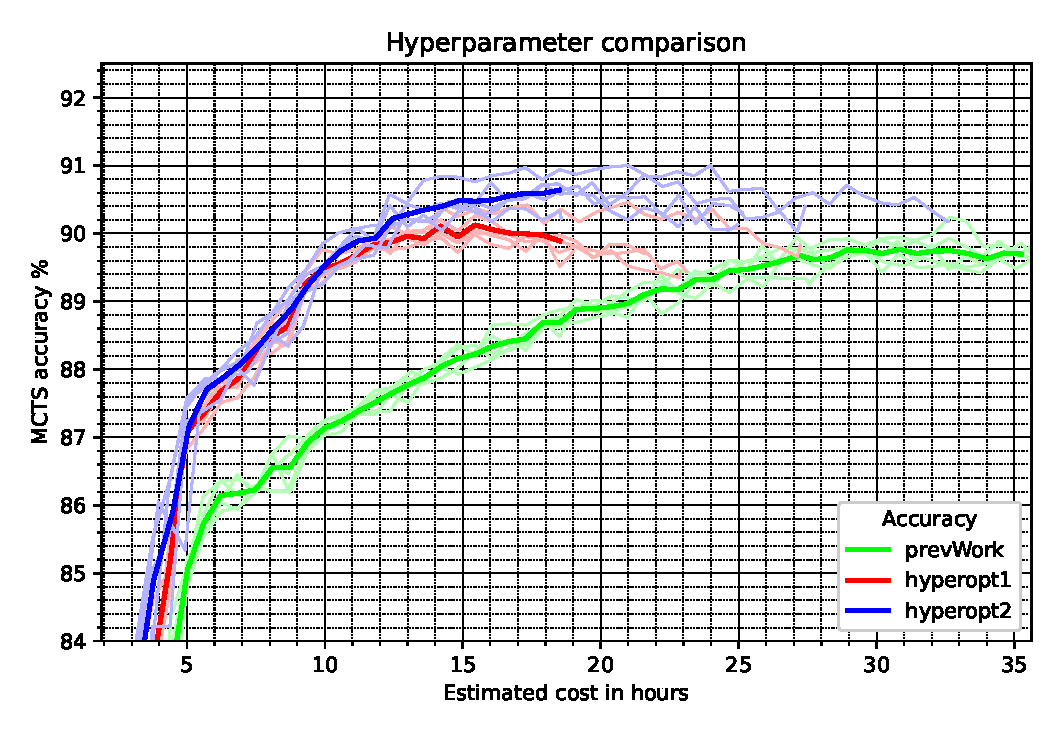
\includegraphics[clip,width=\columnwidth]{hyper_compare}
\caption{Results of the runs to determine a good hyperparameter set. Mean is only calculated until the first of the single runs stops showing improvements.}
\label{fig:hyper_compare_results}
\end{figure}


It can be seen that the results of the parameters taken from previous works fall substantially behind the values found via bayesian optimization. This is likely due to the fact that previous work was on other games, 
using different implementation details, such as different tree sizes, iteration sizes, network sizes or other differences.

The hyperparameter set hyperopt2 is used for all further experiments.

\subsubsection{Evaluation of training costs}

The goal of my work is to identify ways to reduce the substantial costs of training using AlphaZero. The majority of GPU capcacity is spent on self-playing games to be used as training material for the neural network.
In all my experiments I train on a single GPU, evaluate newly produced networks on another single GPU and run self-play workers on a p2p cloud service\footnote{\url{https://vast.ai}} using up to 20 GPUs of various types.

This huge inbalance between training hardware and self-play hardware can be seen in related work as well, e.g. \cite{AlphaZero}[Silver et. al.] used 5000 first-generation TPUs for self-play and 16 second-generation TPUs 
to learn play Chess on super-human, and potentially even super-classical-engine, level within hours. Similarly \cite{wu2019accelerating}[David J. Wu] used up to 24 V100 GPUs to produce self-play training examples to feed a single V100 GPU training data for neural network training to play Go.

The bulk of the training cost consequently lies in the self-play workers. For my experiments I will use this fact to simplify the training cost measurement by ignoring the costs of the training and only measure the time needed to generate self-play games.

Since my main source of computational resources for self-play is a p2p cloud service which provides unreliable but cheap GPU time I am not using a constant number of GPU workers between experiments or often even change the number of workers during training.

After an experiment is completed a benchmarking program is run on a reference machine using the produced networks and measures how much time is needed on average 
to play a single move. This value is then used to estimate the cost of the actual number of moves that were played by the self-play workers during the experiments.

This reference machine uses a single Nvidia RTX 2070S, which is saturated to $100\%$ load by the benchmark. Thus all self-play cost of my experiments is stated as estimated self-play time on that machine and bottlenecked by GPU capcacity on it.


\subsubsection{Results}

As a first baseline I have implemented AlphaZero with only very few modifications, as a minimal baseline.

\subsection{Extended Baseline} \label{s:exexp}

\subsubsection{Remove duplicate positions}

\subsubsection{Cyclic learning rate}

\subsubsection{Improved training window}

\subsubsection{Playout Caps}

\subsubsection{Improving the network structure}



\subsection{Novel improvements}
\subsubsection{Evolutionary hyperparameters}
\subsubsection{Playing games as trees}
\subsubsection{Automatic auxilary features}





\pagebreak

% -- Literaturverzeichnis --------

\bibliographystyle{plain}     % nummeriere Zitate [1], [2], ...

% Quellenangaben stehen in einer separaten BibTeX-Datei Seminararbeit.bib
\bibliography{document}

\end{document}
